\section{Serwer}

Klient webowy uruchamiany w przeglądarce internetowej na urzadzeniu mobilbym użytkownika końcowego łączy się z serwerem przez sieć\footnote{Diagram komponentów w dodatku \ref{app:netwo}}, który odpowiada za poprawne działanie systemu. Korzystając z nowych możliwości przeglądarek internetwoych zaimplementowano dwustronną komunikację (ang. \emph{full duplex communication}) przy uzyciu mechanizmu \emph{Web Sockets}\cite{websockets-rfc} opisaną w podsekcji \ref{subsub:websockets}. Dla urządzeń nie wspierających Web Sockets, przy użyciu biblioteki \emph{Socket.io} (opisanej w podsekcji \ref{subsub:socketio}) dostępne są inne mechanizmy (przegląd w podsekcji \ref{sub:communication}) dwustronnej komunikacji nie wykazujące tak szybkiego działania.

\subsection{Komunikacja między klientem webowym, a serwerem}
\label{sub:communication-methods}

W obu aplikacjach, zarówno grze PONG, jak i pilocie sterującym zdalnym monitorem komunikacja między rozproszonym systemem jest oparta o asynchroniczną wymianę komunikatów (ang. \emph{Asynchronous Message-oriented middleware - MOM})\cite{message-oriented-middleware}.

Dodatkowo przeprowadzano dywagację na temat skalowania stworzonego systemu opisaną w podsekcji \ref{subsub:scalability}. W obliczu skalowalności klienci łączą się do centralnego serwera, który rozdysponuje ruch sieciowy pomiędzy dostępne serwery (ang. \emph{nodes}) obsługujących żądania. W kontekście rozproszenia systemu, architektura MOM polega na asynchronicznem modelu wymiany komunikatów, w przeciwieństwie do modelu żądanie-odpowiedź (\emph{request-response model}). W asynchronicznych systemach kolejki komunikatów pełnią rolę tymczasowego bufora, kiedy odbiorca wiadomości jest zajęty lub niepodłączony do sieci. W dodatku istnieje możliwość stworzenia kolejek trwałych (ang. \emph{persistent queues}), w których wiadomości są zapisywane w pamięci trwałej (np. na dysku) zachowania ich kopii, dzięki czemu nadawca i odbiorca wiadomości nie musi być dostępny w sieci w tym samym czasie - mechanizm ten nazywany jest asynchroniczną dostawa (ang. \emph{asynchronous delivery}). Oznacza to, że gdy odbiorca wiadomości jest niedostępny, wysyłający wiadomości może pracować, a wiadomości zostaną odłożone w kolejce celem późniejszej dostawy, kiedy odbiorca będzie dostępny.

\begin{figure}[H]
  \caption[Model asynchronicznej interakcji w systemach opartych o wymianę komunikatów]{Model asynchronicznej interakcji w systemach opartych o wymianę komunikatów}
  \centering
    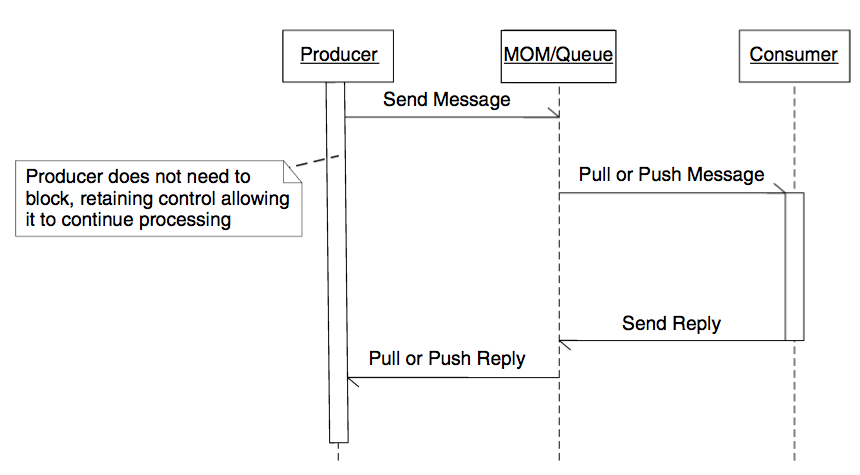
\includegraphics[width=\linewidth]{mom-flow.png} \\
    Diagram UML przepływu przedstawiający model producenta i konsumenta wiadomości połączonego przez system kolejek, źródło\cite{message-oriented-middleware}
\end{figure}

\begin{figure}[H]
  \caption[Schemat działania kolejki w systemach opartych o wymianę komunikatów]{Schemat działania kolejki w systemach opartych o wymianę komunikatów}
  \centering
    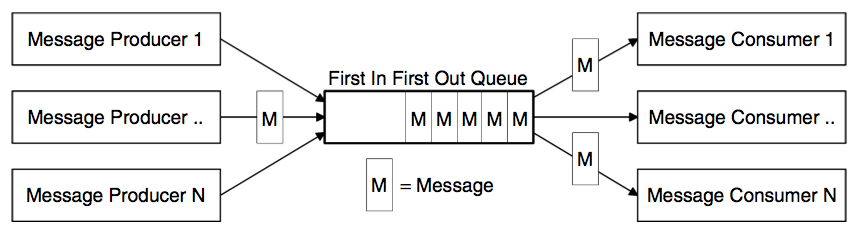
\includegraphics[width=\linewidth]{mom-queue.png} \\
    Diagram przedstawiający model producenta i konsumenta wiadomości połączonego przez system kolejek FIFO, źródło\cite{message-oriented-middleware}
\end{figure}

\subsection{Mechanizmy komunikacji}
\label{sub:communication-methods}

Protokół HTTP\footnote{Hypertext Transfer Protocol} przewiduje komunikację inicjowaną przez klienta do serwera\cite{http-rfc}. Klient wysyła żądanie (ang. \emph{request}) złożoną z nagłówków (ang. \emph{headers}) oraz treści (ang. \emph{body} lub \emph{content}), natomiast serwer zwraca odpowiedź również w postaci nagłówków oraz treści. Każde żądanie jest bezstanowe, swego rodzaju transakcją, to znaczy, że nie zależy od poprzedniego, ani kolejnego. Aby zapewnić transakcyjność stosuje się mechanizmy podtrzymania sesji użytkownika za pomocą przesyłania w nagłówkach ciasteczek zawierający unikatowy identyfikator sesji znany zarówno po stronie klienta, jak i serwera - tym sposobem serwer jest w stanie zidentyfikować następujące po sobie bezstanowe żądania. Istotnym minusem w kontekście prowadzenia komunikacji w protokole HTTP jest to, że serwer nie może zainicjować wysłania danych do przeglądarki, bowiem połączenie jest zamykane zaraz po odesłaniu odpowiedzi. Komunikacja jest jednostronna (ang. \emph{half-duplex communication}).

Przykładowe zapytanie:
\lstset{language=Octave}
\begin{lstlisting}
GET /path/file.html HTTP/1.1\r\n
Host: www.host1.com:80\r\n
\r\n
\end{lstlisting}

Przykładowa odpowiedź:
\lstset{language=Octave}
\begin{lstlisting}
HTTP/1.1 200 OK\r\n
Date: Fri, 31 Dec 1999 23:59:59 GMT\r\n
Content-Type: text/plain\r\n
Transfer-Encoding: chunked\r\n
\r\n \#\# oznacza pusta linie
TUTAJ TRESC
\end{lstlisting}

Aby zapewnić komunikację dwustronną (ang. \emph{full-duplex communication}) (tj. aby serwer mógł wysyłać wiadomości do przeglądarki internetowej w trybie \emph{server push}) stosuje się wiele zabiegów, znanych pod pojęciem komety (ang. \emph{Comet}), których przegląd jest zamieszczony poniżej. Inne znane nazwy tożsame z Comet: \emph{Ajax Push},\footnote{ICEfaces.org [Data dostępu: 27 grudnia 2013]} \emph{Reverse Ajax}\footnote{Crane, Dave; McCarthy, Phil (Lipiec 2008). \emph{Comet and Reverse Ajax: The Next Generation Ajax 2.0}. Apress. ISBN 1-59059-998-5}, \emph{Two-way-web}, \emph{HTTP Streaming}, \footnote{Mahemoff, Michael (Czerwiec 2006). \emph{Web Remoting}. Ajax Design Patterns. O'Reilly Media. s. 19; 85. ISBN 0-596-10180-5}, oraz \emph{HTTP server push}\footnote{Double, Chris (2005-11-05). \emph{"More on Ajax and server push". Different ways of doing server push.}}.

\subsubsection{Komunikacja HTTP persistent connection}
\label{subsub:http-persistent-connection}

Protokół HTTP w wersji 1.0 umożliwia tworzenie stałych połączeń (ang. \emph{persistent connection}) przez przesłanie nagłówka Connection: Keep-Alive, serwer w ramach odpowiedzi odsyła ten sam nagłówek, a od wersji protokołu 1.1 Keep-Alive jest uznawane za domyślne i nie jest konieczne wysłanie nagłówka. Otwarte połączenie przez przeglądarkę internetową nie zamyka go po tuż otrzymaniu odpowiedzi od serwera, a podtrzymuje je mogąc wysłać w ramach niego kilka żądań. Optymalizacja ma na celu zmniejszenia czasu wykonywania żądań o czas otwarcia połączenia po stronie przeglądarki internetowej oraz serwera. Korzyści jest znacznie więcej:

\begin{itemize}
	\item mniejsze zużycie procesora i pamięci operacyjnej,
	\item możliwość wykonania kilku żądań i odpowiedzi jedno po drugim (ang. \emph{pipelining}),
	\item zmniejszenie ruchu sieci (mniej połączeń TCP),
	\item zmniejszone opóźnienie (ang. \emph{latency}) związane z nawiązaniem połączenia z odległym hostem,
	\item w przypadku żądań HTTPS\footnote{Secured HTTP, połączenie podpisane certyfikatem SSL} zmniejsza się liczba obiegów sieci (ang. \emph{network round-trips}) celem wymiany kluczy publicznych oraz certyfikatu.
\end{itemize}

\begin{figure}[H]
  \caption[HTTP Persistent Connection]{HTTP Persistent Connection}
  \centering
    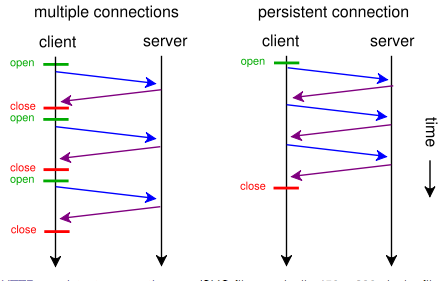
\includegraphics[scale=0.75]{http-persistent-connection.png} \\
    Rysunek przedstawia wysyłanie kolejnych żądań HTTP w ramach osobnych połączeń (domyślnie HTTP 1.0, po lewej stronie) oraz w ramach jednego połączenia (persistent connection, po prawej).
\end{figure}

\subsubsection{HTTP Server Push, Pushlet, JSONP Pooling oraz Script Tag long pooling, Hidden IFRAME}

Korzystając z możliwości użycia \emph{persistent connections} (opisanego w podsekcji \ref{subsub:http-persistent-connection}) powstały mechanizmy umożliwiające komunikację ze strony od serwera do klienta w trybie push:

\begin{description}
  \item[HTTP Server Push] \hfill \\
  Mechanizm polega na tym, że klient inicjuje żądanie, serwer natomiast podtrzymuje je w trybie zawieszonym (nie odsyła odpowiedzi, połączenie pozostaje otwarte), a gdy wystąpi zdarzenie, może zostać ono wysłane do klienta w trybie natychmiastowym. Jeżeli zachodzi zdarzenie, a klient nie jest podłączony, może zostać dodane do kolejki do wysłania przy następnym żądaniu klienta. Po otrzymaniu odpowiedzi i zerwaniu połączenia klient inicjuje nowe żądanie powtarzając cały proces w pętli. Zwalnia to z konieczności periodycznego sprawdzania, czy zaszły jakieś zdarzenia na serwerze poprzez odpytywania serwera (ang. \emph{pooling}).

  \begin{figure}[H]
    \caption[Zasada działania HTTP Server Push]{Zasada działania HTTP Server Push}
    \centering
      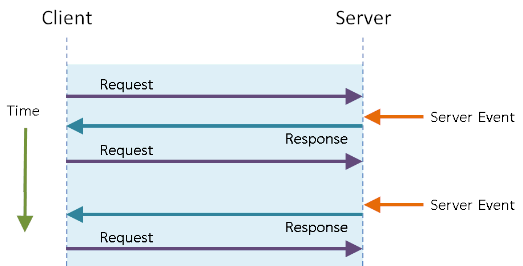
\includegraphics[scale=0.75]{http-server-push.png}
  \end{figure}

  \begin{figure}[H]
    \caption[Porównanie HTTP Pooling oraz HTTP Long Pooling]{Porównanie HTTP Pooling oraz HTTP Long Pooling}
    \centering
      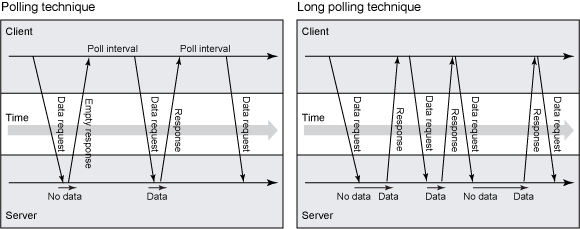
\includegraphics[scale=0.65]{http-pooling-vs-longpooling.jpg}
  \end{figure}

  \item[Pushlet] \hfill \\
  Podejście polegające na podtrzymaniu zainicjowanego połączenia przez klienta w trybie zawieszonym w stanie ciągłego ładowania odpowiedzi (serwer nigdy nie zamyka połączenia). Umożliwia to ciągłe dostarczanie treści do odpowiedzi, która jest interpretowana przez przeglądarkę, np w postaci kodu JavaScript osiągając w ten sposób możliwość wysyłania odpowiedzi z serwera do klienta. W ten sposób po stronie klienta nie jest konieczne uruchomienie appletu Java lub kodu Flash, które dostarczając opcję otwarcia połączenia, ale wymagają zezwolenia od użytkownika.

  \item[XHR Pooling] \hfill \\
  Możliwe jest wykorzystanie obiektu \lstinline{XMLHttpRequest} (\emph{XHR})\cite{xhr-rfc} wykorzystywane w aplikacjach AJAX (ang. \emph{Asynchronous JavaScript and XML}), który umożliwia asynchroniczne odbieranie framgmentow treści strony bez konieczności odświeżenia całej jej zawartości (ponowienia żądania i odpowiedzi). Dane mogą być odbierane w dowolnym formacie, co umożliwia wykorzystanie mechanizmu Comet.\\

  W 1995 roku przeglądarka Netscape Navigator wprowadziła mechanizm który umożliwił serwerowi odświeżanie zawartości obrazka lub kodu HTML wysyłając odpowiedź jako wieloczęściową (ang. \emph{multipart response}) oznaczając ją nagłówkiem

\lstinline{Content-type: multipart/x-mixed-replace}\cite{xhr-rfc}

  Po stornie serwera, każde zdarzenie, które ma być wysłane do klienta jest kolejną częścią odpowiedzi HTTP, odbierane po stronie klienta i interpretowane w wywoływanej funkcji wskazanej jako callback \lstinline{onreadystatechange} wykonywanej za każdym razem, gdy pojawią się nowe dane. Umożliwia to dosyłanie dowolnych porcji danych.

  \item[Hidden IFRAME] \hfill \\
  Technika znana również pod nazwą \emph{forever frame}, polegająca na umieszczeniu w kodzie strony www ukrytej ramki (umożliwiającej wstawienie dokument HTML pochodzący z innej strony internetowej) wykorzystującej mechanizm Pushlet. Gdy wystąpi zdarzenie na serwerze, może ono zostać wysłane jako treść odpowiedzi w postaci tagu HTML
  \lstinline{<script>}
  wypełnionego treścią wykonywalnego kodu JavaScript, który jest natychmiastowo interpretowany przez przeglądarkę. Dokument HTML przyrasta o nowe tagi \lstinline{<script>}. Podstawową zaletą tego rozwiązania jest to, że jest obsługiwane przez każdą przeglądarkę.

  \item[Script Tag long pooling] \hfill \\
  Wszystkie wcześniej wymienione sposoby komunikacji w trybie push od strony serwera wykorzystujące protokół HTTP nie są zdolne do wykonania żądania inicjującego przez klienta poza domenę ze względu na \emph{Same Origin Policy}, bowiem nie można wykonywać połączeń XHR poza domenę\footnote{SLDs - second-level domains} oraz przechwytywać zdarzeń JavaScript z ramki IFRAME z innej domeny. Istnieje sposób na wczytywanie danych spoza domeny za pomocą wczytywania kodu javascript tagiem \lstinline{<script>}, który może wskazywać dowolny adres url wykorzystując technikę Pushlet oraz doładowywać fragmentu kodu JavaScript natychmiastowo wykonywane po stronie przeglądarki.
  
  \item[JSONP Pooling] \hfill \\
  Oparta na technice \emph{Script Tag long pooling} polegająca na doładowywaniu kodu JavaScript zawierającego dane w postaci JSON\footnote{JSON - JavaScript Object Notation} przekazywane jako argument wskazanej wcześniej funkcji w postaci obiektu JavaScript.
  
  Przykład wywołania JSONP Pooling:
\lstset{language=HTML}
\begin{lstlisting}
  <script type="application/javascript"
     src="http://example.com/?functionName=parseResponse">
  </script>
\end{lstlisting}
  
  Jako argument zapytania zostanie wysłana nazwa funkcji, którą serwer umieszcza w odpowiedzi. Jako treść kodu JavaScript wywołuje wskazaną funkcję. Przykładowa odpowiedź serwera:

\lstset{language=JavaScript}
\begin{lstlisting}
   parseResponse({"Name": "Foo", "Id": 1234, "Rank": 7});
\end{lstlisting}

\end{description}

\subsubsection{Metody oparte o wykorzystanie Flash i Java Applets}

Wykorzystując możliwości osadzanych niewidocznych (lub małych, 1x1 pikseli\footnote{one-pixel element}) elementów Flash oraz appletów Java zapewnia się mechanizmy otwierające połączenie TCP bezpośrednio z tych elementów, a komunikacja z przeglądarką internetową odbywa się za pomocą wywoływania funkcji JavaScript z przekazywanymi danymi. Niestety, Flash oraz applety Java nie są wspierane przez przeglądarki na urządzeniach mobilnych, a każda interakcja często jest poprzedzona zgodą klienta.

\subsubsection{Web Sockets}
\label{subsub:websockets}

Opisane metody w sekcji \ref{sub:communication-methods} nie zapewniają komunikacji dwukierunkowej (ang. \emph{full-duplex} lub \emph{bi-directional communication}) za pomocą jednego połączenia TCP. Wychodząc na przeciw oczekiwaniom twórców witryn www czasu rzeczywistego wprowadzony został mechanizm \emph{Web Sockets} ustandaryzowany przez IETF\footnote{Internet Engineering Task Force} w dokumencie RFC-6455\cite{websockets-rfc} umożliwiający nawiązanie połączenia TCP wprost z przeglądarki internetowej. W chwili obecnej większość przeglądarek internetowych wspiera standard Web Sockets\cite{caniuse-websockets}, w tym przeglądarki na urządzeniach mobilnych.

\begin{figure}[H]
  \caption[Zasada działania protokołu Web Sockets]{Zasada działania protokołu Web Sockets}
  \centering
    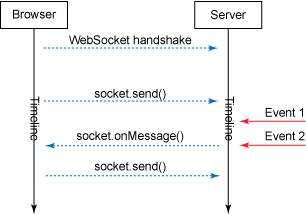
\includegraphics[scale=0.75]{websockets-flow.jpg}
\end{figure}

Protokół Web Sockets został zaprojektowany dla przeglądarek internetowych, natomiast może być użyty w jakiejkolwiek aplikacji. Opiera się na protokole HTTP, ale tylko do czasu przełączenia za pomocą \emph{Upgrade Request} na właściwą wymianę danych, by przystąpić do etapu \emph{handshake}. Aby ustanowić połączenie w protokole Web Sockets, klient wysyła żądanie w protokole HTTP:

\lstset{language=Octave}
\begin{lstlisting}
GET /chat HTTP/1.1
Host: server.example.com
Upgrade: websocket
Connection: Upgrade
Sec-WebSocket-Key: dGhlIHNhbXBsZSBub25jZQ==
Origin: http://example.com
Sec-WebSocket-Protocol: chat, superchat
Sec-WebSocket-Version: 13
\end{lstlisting}

Klient wysyła nagłówek \lstinline{Sec-WebSocket-Key} o wartości będącej wartością losową zakodowaną jako base64\footnote{Jeden ze sposobów kodowania ciągów bajtów}.

Serwer wysyła odpowiedź \emph{101 Switching Protocols}:

\lstset{language=Octave}
\begin{lstlisting}
HTTP/1.1 101 Switching Protocols
Upgrade: websocket
Connection: Upgrade
Sec-WebSocket-Accept: s3pPLMBiTxaQ9kYGzzhZRbK+xOo=
Sec-WebSocket-Protocol: chat
\end{lstlisting}

W odpowiedzi na nagłówek \lstinline{Sec-WebSocket-Key} serwer odsyła w odpowiedzi nagłówek \lstinline{Sec-WebSocket-Accept} o wartości będącą równą:

\vspace*{1\baselineskip}
\lstinline{base64(sha1( klucz ))}
\vspace*{1\baselineskip}

Gdzie klucz to sklejenie ciągu znaków pochodzących z wartości \lstinline{Sec-WebSocket-Key} oraz stałej, ustalonej wartości \lstinline{258EAFA5-E914-47DA-95CA-C5AB0DC85B11}.

Od tego momentu rozpoczyna się transmisja w protokole Web Socekts, grze przesyłane są ramki w trybie full-duplex:

\begin{figure}[H]
  \caption[Ramka protokołu Web Sockets]{Ramka protokołu Web Sockets}
  \centering
    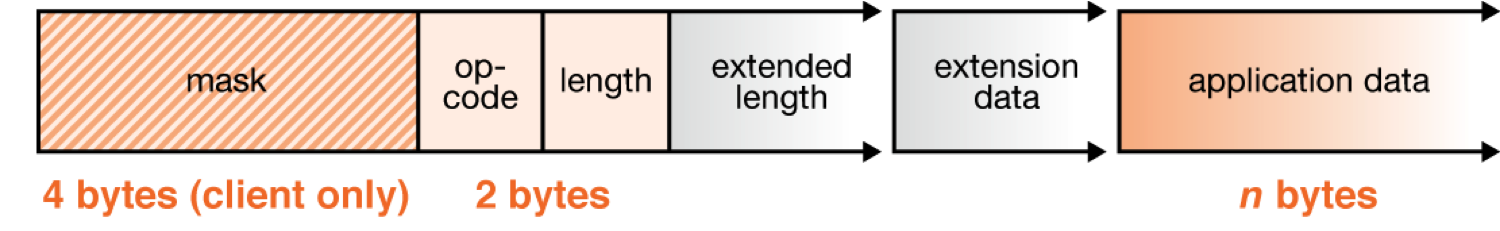
\includegraphics[scale=0.65]{WebSocketFrame.png}
\end{figure}

\subsection{Wykorzystana technologia}

\subsubsection{Synchroniczny i imperatywny model programowania}

\subsubsection{Asynchroniczny i funkcyjny model programowania}

\subsubsection{Zasada działania Node.js}

\subsubsection{Socket.io}
\label{subsub:socketio}

\subsubsection{Skalowanie}
\label{subsub:scalability}

% http://book.mixu.net/node/ch13.html